
% --------------------------------------------------------------
% This is all preamble stuff that you don't have to worry about.
% Head down to where it says "Start here"
% --------------------------------------------------------------
 
\documentclass[12pt]{article}

\usepackage{booktabs} 
\usepackage{graphicx}
\usepackage[margin=1in]{geometry} 
\usepackage{float}

% \usepackage{amsmath,amsthm,amssymb}

\usepackage{Sweave}
\begin{document}
\Sconcordance{concordance:program_template.tex:program_template.Rnw:1 15 1 1 0 329 1}

 
% --------------------------------------------------------------
%                         Start here
% --------------------------------------------------------------
 
\title{Research Replicability \\and \\Workflow Management}
\author{Yann Dorville\\UQAM}

\maketitle

\section{Research Question}
The wage gap has been widely studied and documented. In this analysis, we will explore it both visually and through a silly regression.

\section{Program Overview}
\begin{enumerate} 
  \item Load and clean data 
  \item Summary statistics
  \item Plot
  \item Regression
\end{enumerate}


\section{Detailed Execution}
\subsection{Load and clean data}
Load the 2016 Census of Population.

\subsubsection*{Subsetting}
Select the columns indicated in table \ref{tab:variable-recoding} and recode them as described.\\
Variables Field of study, occupation, industry, and labor force status do not require recoding at this stage.

\subsubsection*{Filtering}
Once the data is loaded, apply the following filters:\\
- Keep only workers who are employed and at work (LFACT = 1).\\
- Remove rows with missing values. This step should be done after recoding.\\
- For the industry, occupation, and field of study variables, exclude values 88 and 99.\\
- For the income variable, exclude values $88888888$ and $99999999$.\\

\subsubsection*{Transformation}
Convert income in thousands\\
Then, compute the occupation$\times$sex specific median.\\
Finally, create additional columns to label variables Field of Study, Industry, and Occupation, as per table \ref{tab:nocs-names}, table \ref{tab:naics-names}, and table \ref{tab:field-study-names}.

\begin{table}[H]
\centering
\caption{Variable Recoding Specifications}
\label{tab:variable-recoding}
\begin{tabular}{@{}lcccc@{}}
\toprule
\textbf{Variable} & \textbf{Variable ID} & \textbf{Recode} & \textbf{Value} \\ \midrule
Age & AGEGRP & 
\begin{tabular}[c]{@{}c@{}}
$x$ $<$ 7\\ 
7 $\leq$ $x$ $\leq$ 9\\ 
10 $\leq$ $x$ $\leq$ 12\\ 
13 $\leq$ $x$ $\leq$ 16\\ 
$x$ $\geq$ 17
\end{tabular} & 
\begin{tabular}[c]{@{}c@{}}
NA\\ 
"Young"\\ 
"Middle"\\ 
"Older"\\ 
NA
\end{tabular} \\ \midrule
Sex & Sex & 
\begin{tabular}[c]{@{}c@{}}
$x$ = 1\\ 
$x$ = 2
\end{tabular} & 
\begin{tabular}[c]{@{}c@{}}
"Female"\\ 
"Male"
\end{tabular} \\ \midrule
Visible Minority & VisMin & 
\begin{tabular}[c]{@{}c@{}}
$x$ $<$ 13\\ 
$x$ = 13\\ 
$x$ $>$ 13
\end{tabular} & 
\begin{tabular}[c]{@{}c@{}}
"Yes"\\ 
"No"\\ 
NA
\end{tabular} \\ \midrule
Education & HDGREE & 
\begin{tabular}[c]{@{}c@{}}
$x$ = 1\\ 
2 $\leq$ $x$ $\leq$ 8\\ 
9 $\leq$ $x$ $\leq$ 13\\ 
$x$ $\geq$ 14
\end{tabular} & 
\begin{tabular}[c]{@{}c@{}}
"None"\\ 
"Medium"\\ 
"High"\\ 
NA
\end{tabular} \\ \midrule
Income & EmpIn & - & - \\ \midrule
Field of Study & CIP2011 & - & - \\ \midrule
Labor Status & LFACT & - & - \\ \midrule
Occupation & NOCS & - & - \\ \midrule
Industry & NAICS & - & - \\
\bottomrule
\end{tabular}
\end{table}


\begin{table}[h]
\centering
\caption{NOCS Classification}
\label{tab:nocs-names}
\begin{tabular}{@{}cc@{}}
\toprule
\textbf{NOCS} & \textbf{Label} \\ \midrule
1 & Management \\
2 & Business \& Finance \\
3 & Sciences \\
4 & Health \\
5 & Social and Education \\
6 & Arts \\
7 & Sales and Services \\
8 & Trades and Transport \\
9 & Primary Industry \\
10 & Manufacturing \\
\bottomrule
\end{tabular}
\end{table}

\begin{table}[h]
\centering
\caption{NAICS Classification}
\label{tab:naics-names}
\begin{tabular}{@{}cc@{}}
\toprule
\textbf{NAICS} & \textbf{Label} \\ \midrule
1  & Agriculture \\
2  & Mining \& Extraction \\
3  & Utilities \\
4  & Construction \\
5  & Manufacturing \\
6  & Wholesale \\
7  & Retail \\
8  & Transportation \\
9  & Information and Cultural Industries \\
10 & Finance \\
11 & Real Estate \\
12 & Professional Services \\
13 & Administrative and Support \\
14 & Education \\
15 & Health Care \\
16 & Arts \& Entertainment \\
17 & Accommodation and Food \\
18 & Other Services \\
19 & Public Administration \\ 
\bottomrule
\end{tabular}
\end{table}

\begin{table}[h]
\centering
\caption{Field of Study Classification}
\label{tab:field-study-names}
\begin{tabular}{@{}cc@{}}
\toprule
\textbf{Field of Study} & \textbf{Label} \\ \midrule
1  & Education \\
2  & Communications \\
3  & Humanities \\
4  & Social Sciences \& Law \\
5  & Business \& Management \\
6  & Life Sciences \\
7  & Mathematics \& Computer Sciences \\
8  & Architecture \& Engineering \\
9  & Agriculture \\
10 & Health \\
11 & Transportation Services \\
12 & Other \\
13 & No Degree \\
\bottomrule
\end{tabular}
\end{table}

\subsection{Summary statistics}
Compute the occupation$\times$sex specific average income and standard deviation.\\
Report the data in a table.

\begin{table}[H]
\centering
\caption{Mean and Standard Deviation of Income by Occupation and Gender}
\label{tab:income_by_gender}
\begin{tabular}{@{}lcc@{}}
\toprule
\textbf{Occupation} & \multicolumn{2}{c}{\textbf{Income Statistics}} \\
 & \textbf{Female} & \textbf{Male} \\
\midrule
Arts & $32.4 \, (\pm 33.0)$ & $43.6 \, (\pm 56.6)$ \\
Business \& Finance & $47.4 \, (\pm 37.1)$ & $75.4 \, (\pm 111)$ \\
Health & $54.2 \, (\pm 40.7)$ & $96.2 \, (\pm 128.5)$ \\
Management & $70.7 \, (\pm 61.7)$ & $101.6 \, (\pm 130)$ \\
Manufacturing & $33.8 \, (\pm 25.7)$ & $55.7 \, (\pm 45.5)$ \\
Primary Industry & $21.2 \, (\pm 22.2)$ & $50.6 \, (\pm 58.5)$ \\
Sales and Services & $25.1 \, (\pm 25.6)$ & $38.6 \, (\pm 53.7)$ \\
Sciences & $66.8 \, (\pm 47.3)$ & $83.1 \, (\pm 77.5)$ \\
Social and Education & $49.4 \, (\pm 40.3)$ & $83.2 \, (\pm 94.0)$ \\
Trades and Transport & $34.1 \, (\pm 27.0)$ & $53.5 \, (\pm 40.7)$ \\
\bottomrule
\end{tabular}
\end{table}



\subsection{Plot}
Create a facetted histogram displaying the distribution of female and male workers in each occupation. That is, for each occupation, overlap two histograms, each corresponding to the income distribution of a gender. Indicate the occupation$\times$gender specific median with a vertical line in each panel.


\begin{figure}[H]
  \centering
  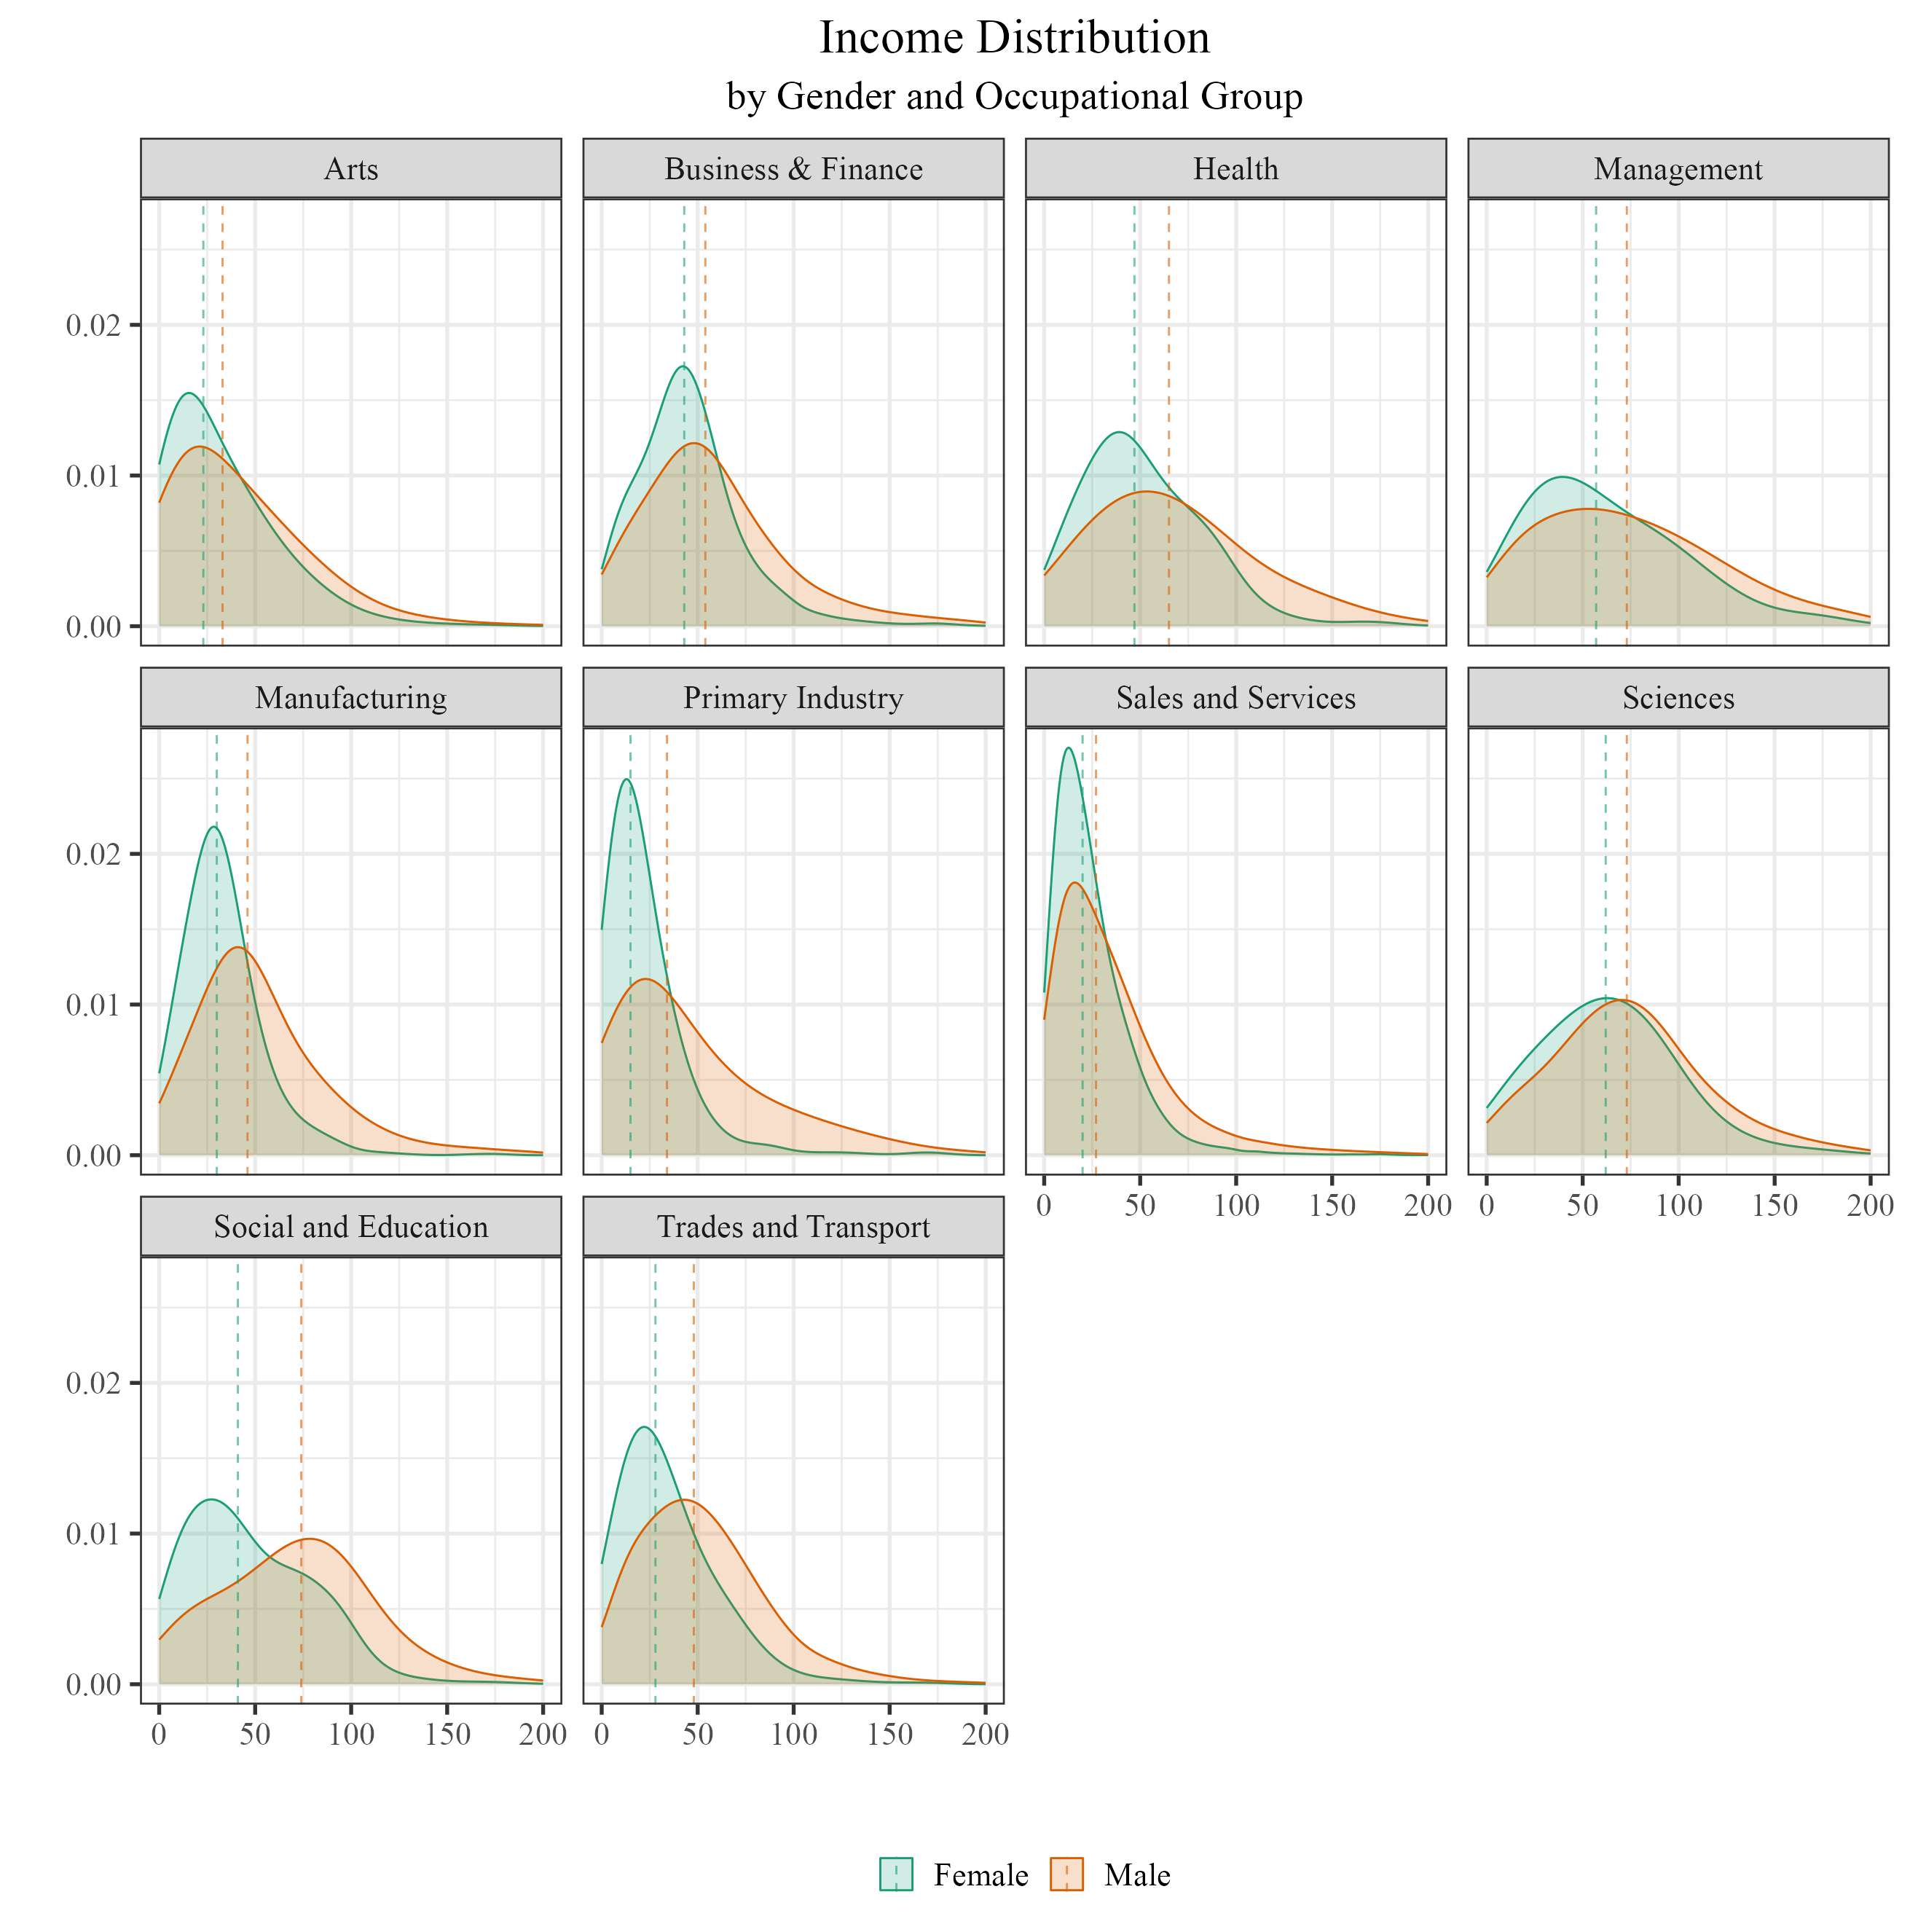
\includegraphics[scale=0.1]{income_distr}
  \caption{Income distribution of female (green) and male (red) Canadian workers in 2016. Dashed lines correspond to the occupation$\times$sex specific medians.}
\end{figure}



\subsection{Regression}
Estimate the following model: $$income = \mu + \beta Sex + \gamma X + \varepsilon$$

\noindent Where $X$ contains controls listed in \ref{tab:controls}

\begin{table}[H]
\centering
\caption{Control variables}
\label{tab:controls}
\begin{tabular}{@{}c@{}}
 \midrule
Age \\
Education \\
Field of Study \\
Visible Minority \\
Occupation \\
Industry \\
\bottomrule
\end{tabular}
\end{table}
 
The results indicate that the factors controlled for in this analysis are not sufficient to explain the gender differences in income.

\begin{table}[ht]
\centering
\caption{Regression Summary (1/2)}
\label{tab:regression-result1of2}
\small
\begin{tabular}{@{}lrrr@{}}
\toprule
\textbf{Variable} & \textbf{Estimate} & \textbf{Std. Error} & \textbf{P-value} \\ \midrule
Intercept & 32.0870 & 1.2665 & $<$ 2e-16 *** \\
\textit{SEX} & & & \\
\quad Male & 20.1871 & 0.2416 & $<$ 2e-16 *** \\
\textit{OCCUPATION} & & & \\
\quad Business and Finance & 11.5574 & 0.7273 & $<$ 2e-16 *** \\
\quad Health & 29.5928 & 0.8958 & $<$ 2e-16 *** \\
\quad Management & 40.7642 & 0.7493 & $<$ 2e-16 *** \\
\quad Manufacturing & 4.0053 & 0.8869 & 6.30e-06 *** \\
\quad Primary Industry & 10.0129 & 1.0850 & $<$ 2e-16 *** \\
\quad Sales and Services & 7.5037 & 0.7306 & $<$ 2e-16 *** \\
\quad Sciences & 17.0535 & 0.7911 & $<$ 2e-16 *** \\
\quad Social and Education & 20.2722 & 0.7678 & $<$ 2e-16 *** \\
\quad Trades and Transport & 5.6019 & 0.7743 & 4.66e-13 *** \\
\textit{FIELD OF STUDY} & & & \\
\quad Architecture and Engineering & 12.1840 & 0.9577 & $<$ 2e-16 *** \\
\quad Business and Management & 11.6885 & 0.9606 & $<$ 2e-16 *** \\
\quad Communications & -3.3413 & 1.1357 & 0.00326 ** \\
\quad Education & 0.8645 & 1.1049 & 0.43398 \\
\quad Health & 10.9971 & 1.0307 & $<$ 2e-16 *** \\
\quad Humanities & -6.2693 & 1.0837 & 7.26e-09 *** \\
\quad Life Sciences & 2.4814 & 1.1307 & 0.02820 * \\
\quad Mathematics and Computer Sciences & 5.4791 & 1.1022 & 6.66e-07 *** \\
\quad No Degree & 3.7068 & 0.9404 & 8.09e-05 *** \\
\quad Social Sciences and Law & 5.7321 & 0.9988 & 9.52e-09 *** \\
\quad Transportation Services & 7.7630 & 1.0477 & 1.27e-13 *** \\
\textit{AGE} & & & \\
\quad Older & 10.0387 & 0.2318 & $<$ 2e-16 *** \\
\quad Young & -18.5711 & 0.2822 & $<$ 2e-16 *** \\
\textit{MINORITY} & & & \\
\quad Yes & -14.5972 & 0.2609 & $<$ 2e-16 *** \\
\textit{EDUCATION} & & & \\
\quad Medium & -25.8503 & 0.2921 & $<$ 2e-16 *** \\
\quad None & -32.0685 & 0.5012 & $<$ 2e-16 *** \\
\bottomrule
\end{tabular}
\end{table}





\begin{table}[ht]
\centering
\caption{Regression Summary (2/2)}
\label{tab:regression-result2of2}
\small
\begin{tabular}{@{}lrrr@{}}
\toprule
\textbf{Variable} & \textbf{Estimate} & \textbf{Std. Error} & \textbf{P-value} \\ \midrule
\textit{INDUSTRY} & & & \\
\quad Administrative and Support & 1.5159 & 0.6514 & 0.01996 * \\
\quad Agriculture & -12.4117 & 0.9247 & $<$ 2e-16 *** \\
\quad Arts and Entertainment & 1.0118 & 0.9028 & 0.26240 \\
\quad Construction & 14.2683 & 0.6270 & $<$ 2e-16 *** \\
\quad Education & 4.4944 & 0.6636 & 1.27e-11 *** \\
\quad Finance & 39.7469 & 0.6393 & $<$ 2e-16 *** \\
\quad Health Care & 3.7464 & 0.6116 & 9.04e-10 *** \\
\quad Information and Cultural Industries & 25.5525 & 0.8192 & $<$ 2e-16 *** \\
\quad Manufacturing & 19.3766 & 0.6005 & $<$ 2e-16 *** \\
\quad Mining and Extraction & 85.0540 & 1.0045 & $<$ 2e-16 *** \\
\quad Other Services & 1.9258 & 0.6536 & 0.00321 ** \\
\quad Professional Services & 22.5766 & 0.6155 & $<$ 2e-16 *** \\
\quad Public Administration & 20.9234 & 0.6221 & $<$ 2e-16 *** \\
\quad Real Estate & 15.8009 & 0.9062 & $<$ 2e-16 *** \\
\quad Retail & 2.9646 & 0.5001 & 3.06e-09 *** \\
\quad Transportation & 14.2057 & 0.6653 & $<$ 2e-16 *** \\
\quad Utilities & 53.4601 & 1.2731 & $<$ 2e-16 *** \\
\quad Wholesale & 23.5877 & 0.6761 & $<$ 2e-16 *** \\
\bottomrule
\end{tabular}
\end{table}


\end{document}
